%%%%%%%%%%%%%%%%%%%%%%%%%%%%%%%%%%%%%%%%%
% Short Sectioned Assignment LaTeX Template Version 1.0 (5/5/12)
% This template has been downloaded from: http://www.LaTeXTemplates.com
% Original author:  Frits Wenneker (http://www.howtotex.com)
% License: CC BY-NC-SA 3.0 (http://creativecommons.org/licenses/by-nc-sa/3.0/)
%%%%%%%%%%%%%%%%%%%%%%%%%%%%%%%%%%%%%%%%%

% \documentclass[paper=a4, fontsize=11pt]{scrartcl} % A4 paper and 11pt font size
\documentclass[11pt, a4paper]{book}
\usepackage[T1]{fontenc} % Use 8-bit encoding that has 256 glyphs
\usepackage[utf8]{inputenc}
\usepackage{fourier} % Use the Adobe Utopia font for the document - comment this line to return to the LaTeX default
\usepackage{listings} % para insertar código con formato similar al editor
\usepackage[spanish, es-tabla]{babel} % Selecciona el español para palabras introducidas automáticamente, p.ej. "septiembre" en la fecha y especifica que se use la palabra Tabla en vez de Cuadro
\usepackage{url} % ,href} %para incluir URLs e hipervínculos dentro del texto (aunque hay que instalar href)
\usepackage{graphics,graphicx, float} %para incluir imágenes y colocarlas
\usepackage[gen]{eurosym} %para incluir el símbolo del euro
\usepackage{cite} %para incluir citas del archivo <nombre>.bib
\usepackage{enumerate}
\usepackage{hyperref}
\usepackage{graphicx}
\usepackage{tabularx}
\usepackage{booktabs}
\usepackage{threeparttable}

\usepackage[table,xcdraw]{xcolor}
\hypersetup{
	colorlinks=true,	% false: boxed links; true: colored links
	linkcolor=black,	% color of internal links
	urlcolor=cyan		% color of external links
}
\renewcommand{\familydefault}{\sfdefault}
\usepackage{fancyhdr} % Custom headers and footers
\pagestyle{fancyplain} % Makes all pages in the document conform to the custom headers and footers
\fancyhead[L]{} % Empty left header
\fancyhead[C]{} % Empty center header
\fancyhead[R]{Francisco Javier Bolívar Expósito} % My name
\fancyfoot[L]{} % Empty left footer
\fancyfoot[C]{} % Empty center footer
\fancyfoot[R]{\thepage} % Page numbering for right footer
%\renewcommand{\headrulewidth}{0pt} % Remove header underlines
\renewcommand{\footrulewidth}{0pt} % Remove footer underlines
\setlength{\headheight}{13.6pt} % Customize the height of the header

\usepackage{titlesec, blindtext, color}
\definecolor{gray75}{gray}{0.75}
\newcommand{\hsp}{\hspace{20pt}}
\titleformat{\chapter}[hang]{\Huge\bfseries}{\thechapter\hsp\textcolor{gray75}{|}\hsp}{0pt}{\Huge\bfseries}
\setcounter{secnumdepth}{4}
\usepackage[Lenny]{fncychap}


\begin{document}

	% Plantilla portada UGR
	\begin{titlepage}
\newlength{\centeroffset}
\setlength{\centeroffset}{-0.5\oddsidemargin}
\addtolength{\centeroffset}{0.5\evensidemargin}
\thispagestyle{empty}

\noindent\hspace*{\centeroffset}\begin{minipage}{\textwidth}

\centering

\includegraphics[width=0.9\textwidth]{logos/logo_ugr.jpg}\\[1.4cm]

\textsc{ \Large TRABAJO FIN DE GRADO}
\vspace{0.2cm}

\textsc{ GRADO EN INGENIERÍA INFORMÁTICA}
\vspace{1cm}

{\Huge\bfseries UltraStar: Song to txt \\}
\noindent\rule[-1ex]{\textwidth}{3pt}

\vspace{3.5ex}
{\large\bfseries Creación automática de archivos para Karaoke}
\end{minipage}

\vspace{2.5cm}
\noindent\hspace*{\centeroffset}
\begin{minipage}{\textwidth}
\centering

\textbf{Autor} 

{Francisco Javier Bolívar Expósito}
\vspace{2.5ex}

\textbf{Director} 

{Juan Julián Merelo Guervós}
\vspace{2cm}


\includegraphics[width=0.3\textwidth]{logos/etsiit_logo.png}\\[0.1cm]
\textsc{Escuela Técnica Superior de Ingenierías Informática y de Telecomunicación}\\
\textsc{---}\\
Granada, junio de 2022
\end{minipage}
\end{titlepage}


	% Plantilla prefacio UGR
	\thispagestyle{empty}

\begin{center}
\large\bfseries
UltraStar: \texttt{\normalfont{\large\bfseries Song2txt}}

Adaptación automática de canciones para juegos de karaoke
\end{center}

\begin{center}
Francisco Javier Bolívar Expósito
\end{center}


\vspace{0.5cm}
\noindent\textbf{Palabras clave}: \textit{Software libre, UltraStar, Python, Desarrollo ágil}
\vspace{0.7cm}

\noindent\textbf{Resumen}

La adaptación de canciones para videojuegos de karaoke es un proceso complejo y manual que requiere conocimientos musicales, lo que provoca que el número de canciones disponibles sea reducido. Aprovechando los avances en inteligencia artificial, gracias a los cuales es posible resolver problemas con sistemas informáticos que anteriormente requerían la intervención de un humano; este trabajo tiene el propósito de facilitar la adaptación de canciones avanzando en su automatización.

Para ello, utilizando un desarrollo ágil, se ha implementado una aplicación en Python que a partir del audio de una canción estima los tonos de cada nota interpretada por el cantante y los guarda en un archivo con el formato estándar UltraStar para videojuegos de karaoke, con una precisión superior a soluciones existentes. Adicionalmente, la librería desarrollada para trabajar con el formato UltraStar puede ser usada independientemente por otros proyectos.


\cleardoublepage

\begin{otherlanguage}{english}


\begin{center}
\large\bfseries 
\texttt{\normalfont\large\bfseries UltraStar: Song2txt}
	
Automatic adaptation of songs for karaoke games
\end{center}

\begin{center}
	\texttt{\normalfont Francisco Javier Bolívar Expósito}
\end{center}


\vspace{0.5cm}
\noindent\textbf{Keywords}: \textit{FLOSS, UltraStar, Python, Agile development}
\vspace{0.7cm}

\noindent\textbf{Abstract}

Adapting songs for karaoke video games is a complex and manual process that requires musical knowledge, which results in a limited number of songs available. Taking advantage of advances in artificial intelligence, thanks to which it is possible to solve problems with computer systems that previously required the intervention of a human; this work aims to facilitate the adaptation of songs by advancing in its automation.

To this end, using agile development, a Python application has been implemented that, from the audio of a song, estimates the tones of each note performed by the singer and saves them in a file with the standard \texttt{UltraStar} format for karaoke video games, with greater precision than existing solutions. Additionally, the library developed to work with the \texttt{UltraStar} format can be used independently by other projects.

\end{otherlanguage}

\cleardoublepage

\thispagestyle{empty}

\noindent\rule[-1ex]{\textwidth}{2pt}\\[4.5ex]

D. \textbf{Juan Julián Merelo Guervós}, Profesor del departamento de Arquitectura y Tecnología de Computadores.

\vspace{0.5cm}

\textbf{Informo:}

\vspace{0.5cm}

Que el presente trabajo, titulado \textit{\textbf{UltraStar: Song to txt}},
ha sido realizado bajo mi supervisión por \textbf{Francisco Javier Bolívar Expósito}, y autorizo la defensa de dicho trabajo ante el tribunal
que corresponda.

\vspace{0.5cm}

Y para que conste, expiden y firman el presente informe en Granada a junio de 2022.

\vspace{1cm}

\textbf{El/la director(a)/es: }

\vspace{5cm}

\noindent \textbf{Juan Julián Merelo Guervós}

\chapter*{Agradecimientos}

Aprovechando el fin de esta etapa académica, me gustaría agradecer a las personas que me han apoyado y gracias a las cuales soy quien soy.

En primer lugar, quiero agradecer el cariño de mi familia, especialmente a mis padres por su apoyo incondicional y a mi hermana por entenderme como nadie y por las pequeñas llamadas de 5 minutos que acaban durando horas.

También quiero dar las gracias a tantos profesores y compañeros de la universidad que no han dudado en prestar su ayuda, enseñándome tanto y compartiendo su pasión por este campo del conocimiento. A su vez, a la comunidad de software libre y a todas las personas que aportan desinteresadamente su granito de arena, confiando en llegar más lejos cooperando que compitiendo. 

Por último, a los \texttt{\normalfont\textit{Mákinas}} y los\texttt{\normalfont\textit{ Checolegas}}, la gente con la que he pasado algunos de los mejores momentos de esta etapa, con un gran corazón y con la que me siento en mi sitio.

Es imposible expresar todo lo que me habéis dado estos años y lo feliz que soy de teneros en mi vida. Un abrazo muy grande para todos.

\vspace*{1cm}



	% Índice de contenidos
	\tableofcontents

	% Índice de imágenes y tablas
	\listoffigures

	% Si hay suficientes se incluirá dicho índice
	\listoftables

	% Introducción 
	\chapter{Introducción}

Este proyecto es software libre, liberado con la licencia AGPLv3 \cite{agpl} y publicado en un repositorio público\footnote{\url{https://github.com/dipzza/ultrastar-song2txt}}.

\section{Motivación}
\label{sec:motivation}

El karaoke es un tipo de entretenimiento consistente en cantar junto a música grabada, normalmente con la ayuda de una pantalla en la que se muestra la letra de la canción e indicaciones de cuando hay que cantar cada parte.

Mucha gente disfruta del karaoke como forma de ocio o diversión, cumpliendo el sueño de ser cantante por unos momentos. Por esta razón, existen multitud de programas dirigidos a los entusiastas del karaoke.

Un tipo de estos programas son los videojuegos de karaoke, que ofrecen todavía más ayuda al mostrar el tono en el que se está cantando y como de lejos se encuentra este del correcto. Además, al medir la precisión con la que se ha cantado la canción permiten competir con otras personas o disfrutar buscando la mejora personal.

Sin embargo, los aficionados de los videojuegos de karaoke tienen que lidiar frecuentemente con un problema cuando quieren cantar su canción favorita: que no esté disponible.

Aunque el desarrollo de programas de software libre y gratuitos tanto de videojuegos de karaoke (\href{https://github.com/UltraStar-Deluxe/USDX}{\textit{UltraStar Deluxe}}, \href{https://github.com/Vocaluxe/Vocaluxe}{\textit{Vocaluxe}}, \href{https://github.com/performous/performous}{\textit{Performous}}...) como de herramientas para la creación de canciones (\href{https://github.com/sarutasan72/Yass}{\textit{Yass}}, \href{https://github.com/UltraStar-Deluxe/UltraStar-Creator}{\textit{UltraStar Creator}}...) ha ayudado al desarrollo de comunidades donde se crean y comparten canciones para videojuegos de karaoke, la mayoría de canciones siguen sin estar disponibles, especialmente aquellas más recientes o menos famosas.

Una causa de que la selección de canciones disponibles sea tan limitada es que el proceso de creación de canciones para videojuegos de karaoke es complejo, largo y requiere conocimientos musicales.


\section{Objetivo}

Este trabajo persigue ayudar en la creación de canciones para videojuegos de karaoke, reduciendo la barrera de entrada para personas sin conocimientos musicales y el tiempo que necesitan invertir aquellas con conocimientos musicales.


Para ello se pretende \textbf{mejorar o integrar los procesos de automatización existentes para la creación de canciones para videojuegos de karaoke.}

\section{Terminología}

\begin{itemize}
	\item{Nota. Representación musical de un sonido, con un tono constante y una duración determinada.}
	\item{Tono. Cualidad de los sonidos que permite su ordenación en una escala relacionada con la frecuencia.}
	\item{Frecuencia fundamental. Aquella que representa el tono simple más bajo presente en una nota.}
	\item{MIDI. Estándar técnico en el que se definen 128 notas por su número, con equivalencias a la nomenclatura estándar inglesa.}
	\item{Pulsación. Unidad básica en música para medir el tiempo. Una sucesión constante divide el tiempo en partes iguales.}
	\item{Pulsaciones por minuto. Unidad empleada para medir el ritmo en música. Equivale al número de pulsaciones que caben en un minuto.}
	\item{Fonema. Unidad sonora mínima que puede distinguir una palabra de otra en un lenguaje dado.}
	\item{Software libre. Aquel cuyo código fuente puede ser estudiado, modificado, utilizado libremente para cualquier propósito y redistribuido con cambios o mejoras.}
	\item{Software privativo. Aquel del cual no existe una forma libre de acceso a su código fuente, en el que uno o varios de los derechos de usar, modificar, compartir modificaciones o el software están restringidos.}
\end{itemize}

	% Descripción del problema y Estado del arte
	\chapter{Descripción del problema y estado del arte}

\section{Descripción del problema}
\label{sec:problemdescription}

Con el fin de facilitar el proceso de añadir canciones a videojuegos de karaoke, se pretende avanzar en la automatización de las tareas relacionadas.

Independientemente del formato utilizado para guardar las canciones, las principales tareas consisten en:

\begin{itemize}
	\item{Encontrar e introducir metadatos, como el título, el artista, las pulsaciones por minuto, etc.}
	\item{Obtener la letra de la canción.}
	\item{Definir las notas interpretadas por el cantante original, con la siguiente información asociada a cada una:}
	\begin{itemize}
		\item{El tono del sonido.}
		\item{El intervalo de tiempo en el que sucede.}
		\item{Los fonemas de la letra correspondientes.}
	\end{itemize}
\end{itemize}

Algunas de las tareas son más complejas o tardan más en completarse. Definir la información de las notas en general es un proceso tedioso debido a la gran cantidad de notas que pueden ser cantadas en una canción (por ejemplo, la canción \texttt{'Rolling in the Deep' de Adele} requiere la definición de más de 500 notas individuales) y, en particular, la asignación de los tonos es especialmente compleja porque requiere de oído musical y un proceso de prueba y error.

¿Debe darse prioridad a la automatización de estas tareas, por ser las más complejas? Es un argumento a tener en cuenta, sin embargo, es importante valorar las soluciones ya existentes para decidir el enfoque del trabajo, analizadas en la siguiente sección.

\section{Estado del arte}

\subsection{Formatos para definir de canciones}
\label{sec:formatcomparison}

Para conocer que formatos son los más usados se han analizado los videojuegos de karaoke actuales.

\begin{table}[h!]
	\begin{threeparttable}
		\caption{Compatibilidad en videojuegos de karaoke.}
		\begin{tabular}{ |c|>{\centering\arraybackslash}m{0.35\textwidth}|c|c|}
			\hline
			\textbf{Videojuego} & \textbf{Plataformas compatibles} & \textbf{Tipo de software} & \textbf{Formato usado} \\
			\hline
			UltraStar Deluxe & Linux, Windows, macOS & Libre & UltraStar \\
			UltraStar Play & Linux, Windows, macOS, Android & Libre & UltraStar \\
			Performous & Linux, Windows, macOS & Libre & UltraStar \\
			Vocaluxe & Windows & Libre & UltraStar \\
			SingStar & PS3, PS4 & Privativo & Desconocido\tnote{1} \\
			Let's Sing 2022 & PS4, PS5, Xbox One, Xbox Series, Nintendo Switch & Privativo & VXLA\tnote{2} \\
			\hline
		\end{tabular}
		\begin{tablenotes}
			\item [1] El formato utilizado es desconocido, solo era posible añadir canciones comprándolas en la tienda online integrada, cerrada en 2020. \url{https://www.eurogamer.net/sony-shutting-down-singstars-servers-at-the-start-of-next-year}.
			\item [2] La única forma oficial de añadir canciones es comprarlas en una tienda online con una oferta reducida, pero existen métodos no oficiales para añadir canciones personalizadas a partir del formato UltraStar.  \url{https://gbatemp.net/threads/tutorial-add-custom-songs-to-lets-sing-2022-from-ultrastar.607817/}.
		\end{tablenotes}
	\end{threeparttable}
\end{table}

De lo anterior se deduce que el estándar de facto en los videojuegos de software libre es el formato UltraStar y, ya sea de forma nativa o a través de un conversor, es compatible con todos aquellos que permiten añadir canciones personalizadas.



\subsection{Automatización de tareas en la creación de canciones}

El programa más popular, \href{https://github.com/UltraStar-Deluxe/UltraStar-Creator}{UltraStar Creator}, guía al usuario en la creación y facilita muchas de las tareas:

\begin{itemize}
	\item{Facilita la obtención de metadatos al ser capaz de extraer los contenidos de un archivo MP3 y detectar las pulsaciones por minuto a partir del audio.}
	\item{Separa automáticamente la letra de la canción en fonemas según el idioma de esta.}
	\item{Facilita definir los intervalos de tiempo en los que ocurren las notas, para ello, se reproduce la canción a una velocidad reducida y el programa pide pulsar una tecla cada vez que el usuario escuche una nota nueva, a partir de esto crea las notas con intervalos de tiempo y fonemas asociados.}
\end{itemize}

Editores como \href{https://github.com/sarutasan72/Yass}{Yass} o el integrado en \href{https://usplay.net/#song-editor}{UltraStar Play} proveen una interfaz adecuada para afinar la temporización de las notas y asignar los tonos correspondientes, pero de modo manual.

Estas herramientas simplifican el proceso de creación, no obstante, ninguna de ellas provee una solución conveniente para la asignación de tonos.

Para automatizar esta tarea el proyecto más prometedor es la aplicación\texttt{ \href{https://github.com/paradigmn/ultrastar\_pitch}{ultrastar-pitch}}, publicada en 2020, que a partir de un archivo con toda la información necesaria excepto los tonos de las notas, completa esta información estimándolos con una red neuronal entrenada por el autor. No hay disponible una evaluación de las prestaciones detallada, el autor comenta que la precisión según el tipo de canción puede estar entre el 30\% y el 90\%. Tras probar experimentalmente el programa queda claro que se encuentra muy lejos de lo deseado, incluso en las canciones en las que mejor funciona (baladas con voz femenina) sigue siendo necesaria una revisión manual para obtener una asignación de tonos correcta.

Aparte de la poca precisión, no hay documentación sobre las técnicas utilizadas y el proceso de instalación requiere instalar programas externos que no están especificados en las instrucciones.


\section{Mejoras al estado del arte}

Actualmente, es necesario buscar y establecer manualmente la letra de la canción y los metadatos que no se tengan en un archivo MP3. Esta información podría proveerse automáticamente a partir de \textit{API} públicas u otros métodos.

Respecto a la asignación automática de tonos sería deseable:

\begin{itemize}
	\item{Mejorar la precisión con técnicas para la estimación de la frecuencia fundamental que representen el estado del arte actual.}
	\item{Favorecer mejoras posteriores al trabajo realizado, documentando los métodos empleados, el proceso de decisión y los resultados obtenidos y desarrollando un código modular fácil de mantener.}
	\item{Simplificar el proceso de instalación y el uso de las herramientas.}
\end{itemize}

Otra carencia del estado del arte es que, aunque es posible simplificar la tarea, se sigue requiriendo un proceso manual para definir los intervalos de tiempo de las notas. Sin embargo, la viabilidad de automatizar esta tarea con las técnicas actuales es debatible y requiere de más investigación. Los avances recientes en sincronización automática de subtítulos con audio \cite{Sub-Sync, Deep-Sync} presentan un retraso medio demasiado alto para los requisitos de un videojuego de karaoke, por lo que un posible acercamiento sincronizando los fonemas de la canción no parece factible.
	
	\chapter{Planificación}
\label{ch:planning}

\section{Desarrollo ágil}
\label{sec:agile}

Con el objetivo de desarrollar software de calidad, flexible y adaptado a las necesidades de los clientes, se han seguido los principios del desarrollo ágil popularizados en 2001 por el manifiesto ágil \cite{beck2001agile}. Algunos de estos principios de acorde a los cuales se ha definido la metodología del desarrollo son:

\begin{itemize}
	\item{Nuestra mayor prioridad es satisfacer al cliente, para ello el desarrollo debe realizarse de forma \textbf{iterativa e incremental}, entregando temprano y continuamente cambios que añadan valor.}
	\item{Hay que buscar \textbf{la excelencia técnica} y seguir buenas prácticas para garantizar la flexibilidad y comprensibilidad del proyecto.}
	\item{El diseño es esencial, pero debe \textbf{evitarse la documentación excesiva}, ya que, conseguir código funcional lo antes posible es el mejor modo de confirmar que se entienden los requisitos del cliente.}
	\item{Es necesario \textbf{revisar el trabajo frecuentemente}, para aprender a hacerlo de manera más eficiente, mantener la calidad del software al detectar fallos y adaptarlo a nuevos requisitos.}
\end{itemize}

Con el propósito de cumplir estos principios se han utilizado una serie de herramientas y técnicas durante todo el proceso de desarrollo, que serán descritas en el resto de secciones del capítulo.

\section{Control de versiones}

El uso de un sistema de control de versiones que lleve un registro de los cambios es fundamental, ya que, permite coordinar el trabajo entre desarrolladores, deshacer cambios incorrectos, mantener distintas versiones del código y un largo etcétera de ventajas. Este tipo de sistemas ayudan a seguir un desarrollo iterativo en el que se compruebe el trabajo frecuentemente, tal y como indican los principios ágiles presentados en la sección \ref{sec:agile}. 

Por este motivo, se ha elegido \textit{Git} como software de control de versiones y GitHub tanto para el alojamiento en un \href{https://github.com/dipzza/ultrastar-song2txt}{repositorio público} como plataforma de organización, colaboración y pruebas.

\section{Análisis de usuarios}

Para empatizar con los usuarios que acabarán usando el proyecto es necesario definirlos claramente, pudiendo así enfocar el proyecto a resolver sus problemas.

Con esta intención, empleando la metodología de personas basadas en roles \cite{role-personas}, se han definido los siguientes roles que describen a un grupo de personas que realizan la misma función.

\begin{enumerate}	
	\item{Creador de canciones para videojuegos de karaoke}
	\begin{itemize}
		\item{Misión: Adaptar canciones para poder incluirlas en los videojuegos de karaoke.}
		\item{Nivel de conocimiento: Manejo medio de ordenadores, el sistema operativo que emplean puede ser \textit{Windows}, \textit{Linux} o \textit{macOS}. Importante diferenciar entre aquellos que tienen conocimientos musicales y los que no.}
		\item{Contexto en el que realiza la función: En su tiempo libre, por lo que pueden dejarla a medias o tener un tiempo limitado para hacerla.}
		\item{Productos de los que es usuario: Las aplicaciones desarrolladas.}
	\end{itemize}
	
		\item{Programador}
	\begin{itemize}
		\item{Misión: Desarrollar con el código del proyecto, ya sea contribuyendo a este o reutilizando partes en otros proyectos.}
		\item{Nivel de conocimiento: Conocimiento experto sobre herramientas de desarrollo y colaboración.}
		\item{Contexto en el que realiza la función: Puede ser en su tiempo libre o como parte de sus tareas, pero suele ser con cierta dedicación sin hacer otras tareas a la vez.}
		\item{Producto de los que es usuario: La organización del proyecto, el código de este y la documentación.}
	\end{itemize}
\end{enumerate}

\section{Historias de Usuario}

Se han creado historias de usuario para especificar las necesidades de los usuarios (y, por lo tanto, los requisitos del proyecto). Son comúnmente utilizadas en el desarrollo ágil, ya que, permiten administrar los requisitos de los usuarios rápidamente sin gran cantidad de documentos formales, facilitando la adaptación a requisitos cambiantes. Cada historia de usuario debe tener las siguientes características \cite{hujj}:

\begin{itemize}
	\item{Identifica el tipo de usuario protagonista de la historia.}
	\item{Está en el dominio del problema, es narrada desde el punto de vista del usuario y expresa el beneficio que obtendría este una vez se implemente la historia de usuario.}
	\item{Para completar la historia de usuario será necesario realizar tareas que provoquen cambios en los productos a entregar}
\end{itemize}

\noindent{Se han definido las siguientes historias de usuario:}

\subsubsection*{\href{https://github.com/dipzza/ultrastar-song2txt/issues/7}{[HU01] Creador Karaoke - Detección de tonos}}\label{sec:hu1}

Como creador de canciones para karaoke quiero poder asignar los tonos de la canción en menos tiempo y con menor dificultad.

\subsubsection*{\href{https://github.com/dipzza/ultrastar-song2txt/issues/8}{[HU02] Creador Karaoke - Búsqueda de metadatos}}

Como creador de canciones para karaoke quiero evitar tener que buscar e introducir manualmente información sobre la canción.


\subsubsection*{\href{https://github.com/dipzza/ultrastar-song2txt/issues/10}{[HU03] Programador - Aplicación modular}}

Como programador querría que cada funcionalidad del proyecto fuera independiente, para poder reutilizar solo aquella que necesite al desarrollar otros programas.

\subsubsection*{\href{https://github.com/dipzza/ultrastar-song2txt/issues/11}{[HU04] Programador - Estudio de prestaciones}}

Como programador me gustaría poder ver pruebas detalladas sobre el rendimiento de las soluciones implementadas, para poder elegir con datos objetivos la solución más adecuada.


\section{Hitos}
\label{sec:hitos}

Siguiendo los principios del desarrollo ágil presentados en la sección \ref{sec:agile} el desarrollo debería realizarse de forma \textbf{incremental}, ya que de esta forma es posible presentar resultados frecuentemente y cambiar o adaptar los requerimientos.

Para ello, se han definido hitos, que describen una serie de \textbf{productos mínimamente viables} (\textit{PMV}) que podrían entregarse. Cada uno es más complejo que el anterior incluyendo todo el desarrollo previo, tiene un criterio de aceptación y avanza hacia el cumplimiento de las historias de usuario.

Adicionalmente, los hitos están compuestos de \textit{issues} definidos y asociados al hito correspondiente en el repositorio de GitHub. Los issues son problemas siempre enmarcados en alcanzar un hito y que, por lo tanto, al ser resueltos avanzan en el cumplimiento de las historias de usuario.

% Añadir enlace a hitos, en los títulos o tal vez uno general aparte

\subsection*{Hito 0: Infraestructura y planificación}

El primer PMV consiste en la planificación inicial y la configuración del repositorio. Para ser aceptado debe contener al menos los siguientes elementos:

\begin{itemize}
	\item{Análisis de usuarios.}
	\item{Historias de usuario.}
	\item{Hitos.}
	\item{Automatización en el repositorio para comprobar la ortografía de la memoria y errores sintácticos y de estilo en el código.}
	\item{Motivación, objetivos y capítulos metodológicos redactados en la memoria.}
\end{itemize}

\subsection*{Hito 1: Arquitectura básica para la detección de notas}

Diseño de las clases básicas necesarias para detectar las notas a partir de un archivo de audio y guardarlas en un formato estandarizado de texto de videojuegos de karaoke. Inicialmente con una solución simple, aunque esta no posea una precisión alta.

Para la aceptación del PMV este debe contener tests para cada clase y al menos las definiciones de las clases y sus funciones. Además, la memoria debe reflejar todas las decisiones tomadas en el proceso.

\subsection*{Hito 2: Evaluación de la detección de notas}

Es necesario proveer un análisis de las prestaciones de las soluciones implementadas. Para aceptar este PMV este debe contener:
\begin{itemize}
	\item{Selección de métricas adecuadas para medir la calidad de la detección de notas}
	\item{Selección o creación de un conjunto de datos para la evaluación}
	\item{Código para realizar la evaluación correspondiente}
	\item{Redacción del Análisis y la comparación de los resultados}
\end{itemize}

\section{Control de la calidad}

Con la intención de construir software de calidad desde el principio, preparado para entregar constantemente, y hacer cumplir la excelencia en el desarrollo del manifiesto ágil \cite{beck2001agile}, se ha aplicado \textbf{integración continua}, fusionando cambios a la línea principal de desarrollo solo una vez que estos pasen por test automatizados altamente estrictos.

Al subir cualquier cambio a GitHub se ejecutan automáticamente las pruebas. Para el código se han configurado las siguientes comprobaciones:

\begin{itemize}
	\item{Errores, adherencia a la guía de estilo PEP8 \cite{pep8} y complejidad del código.}
	\item{Test unitarios, de integración y de cobertura. Los tests han de definirse cubriendo un único caso lógico por cada test, lo que permite saber con precisión que funciona exactamente y que no, y cubriendo la mayor cantidad posible de casos lógicos. Para aceptar un PMV al menos el 85\% de su código debe estar cubierto por tests.}
	\item{Correcta instalación del proyecto y sus dependencias}
\end{itemize}

Además, para la memoria escrita en LaTeX, teniendo en cuenta el texto \textbf{en inglés y en español}:
\begin{itemize}
	\item{Compilación del PDF sin errores.}
	\item{Corrección ortográfica y gramatical.}
	\item{Reglas de estilo en la redacción.}
\end{itemize}


\section{Resumen de la metodología}

Una vez presentadas las herramientas y técnicas usadas es posible definir la metodología aplicada explicando el orden de los procesos.

Se empieza la planificación realizando un \textbf{análisis de usuarios} para empatizar, se definen los requisitos del proyecto con \textbf{historias de usuario} (que pueden cambiar a lo largo del desarrollo) y creamos \textbf{hitos} para tener un horizonte de trabajo hacia los PMV, que pueden ser ampliados si tras ser cumplidos quedan historias de usuario sin resolver. Una vez finalizada esta planificación inicial, el desarrollo continúa con los siguientes pasos en bucle. 

Se genera una ramificación del código principal en la que implementar una nueva funcionalidad, teniendo en cuenta los \textit{issues} que componen el hito en el que estemos trabajando.

Se avanza en esta nueva rama con \textit{commits} (conjuntos de cambios confirmados). Cada uno de los \textit{commits} tiene asociado un \textbf{mensaje corto y conciso} que explica los cambios, con \textbf{referencia a un \textit{issue}} para saber que se pretende resolver y un \textbf{emoticono} (según el estándar definido en \url{https://gitmoji.dev/about}) que facilita identificar la intención del \textit{commit} con un vistazo.

Una vez la nueva función está implementada y la rama pasa todos los \textbf{tests de integración continua} se hace una petición para integrar los cambios en la rama principal con un \textbf{\textit{Pull Request}} en GitHub. En este momento, los cambios son revisados por el resto del equipo (en este caso, normalmente, por el tutor) que puede ver fácilmente que se cumplen los tests y la intención de los cambios gracias a la historia lineal y descriptiva que se forma con los mensajes de los \textit{commits}.

Los revisores inician una \textbf{conversación independiente por cada sugerencia} o pregunta realizada en la que se cita las líneas de texto afectadas, lo que permite mantener un diálogo ordenado y claro. Una vez todas las cuestiones que surgen en la revisión son resueltas, los cambios son integrados en la rama principal y automáticamente se cierran los \textit{issues} afectados.

\section{Estimación de costes}


\begin{table}[H]
	\centering
	\begin{tabular}{| l | l | r |}
    		\hline
        \textbf{Concepto} & \textbf{Detalle} & \textbf{Coste} \\
        \hline
        Material utilizado	& Ordenador, monitor y periféricos & Amortización* 312 €/año\\
        Personal contratado 	& Ingeniero de ML Junior	& 1500-2000 €/mes \\
        Recursos software 	& Software libre gratuito & 0 € \\
        Recursos en la nube 	& GitHub plan gratuito & 0 € \\
        \hline
        Coste total 			& 3 meses de desarrollo & 4740 € - 6240 € \\
        \hline
	\end{tabular}
	\caption{Costes estimados del proyecto.}
\end{table}

*Amortización aplicando el coeficiente máximo de amortización lineal para el grupo ''Equipos para procesos de información'', que es del 25\% durante 4 años. Se incluye todo el equipo informático como conjunto operativo. Coste de compra total 1200 €, 950 € ordenador, 150 € monitor, 100 € periféricos. \cite{lis}.

	\chapter{Implementación}

La implementación del software se ha dividido en hitos tal y como se explica en la sección \ref{sec:hitos}. Estos han sido definidos en GitHub
y cada uno de ellos contiene un grupo de \textit{issues} que se corresponden con las distintas
mejoras que se han ido incorporando al software a lo largo de su desarrollo.

\section{Hito 0. Infraestructura y planificación}

Se realizó la planificación inicial que se puede encontrar redactada en el capítulo \ref{ch:planning} y organizada en el \href{https://github.com/dipzza/ultrastar-song2txt}{repositorio} del proyecto. Además, se configuraron las siguientes herramientas.


\subsection{Integración Continua}

Se consideraron varios servicios que permiten \textbf{automatizar los procesos de integración continua} en la nube, con la condición de que dispongan de planes gratuitos para proyectos de código abierto y buscando el servicio más sencillo de integrar con el repositorio del proyecto en GitHub.

Tanto Travis CI,  Circle CI y GitHub Actions ofrecen planes gratuitos. Se considera que GitHub Actions es el servicio que mejor cumple las características deseadas, debido a su integración dentro de la propia interfaz de GitHub, la facilidad de configuración y la posibilidad de reusar flujos de trabajo públicos (también llamados acciones). Los otros servicios poseen ventajas, como soporte para otras plataformas en las que alojar el código o diferencias en los precios de los planes de pago, pero para este proyecto se consideran irrelevantes.

Utilizando el servicio escogido se han configurado una serie de flujos de trabajo que son ejecutados cada vez que se introducen cambios en cualquier rama de desarrollo.

\subsubsection{Memoria}

\paragraph*{Compilación de archivos de LaTeX.}

La memoria del trabajo ha sido escrita con LaTeX, un sistema de composición de textos comúnmente usado en artículos académicos, tesis y libros técnicos por su calidad tipográfica y amplias capacidades.

Es necesario compilar los archivos de LaTeX para obtener el documento final. Por ello, se ha configurado un flujo de trabajo para \textbf{comprobar que la compilación se completa sin errores}. El flujo realiza un paso adicional si la rama principal de desarrollo está afectada (ya sea por introducir cambios o por hacerse un \textit{pull request} a esta) que \textbf{almacena el documento final generado}.

\paragraph*{Corrección de la memoria.}

Para asegurar una correcta redacción de la memoria se ha utilizado la herramienta de software libre \href{https://github.com/sylvainhalle/textidote}{TeXtidote}. A diferencia de otras herramientas que solo revisan la ortografía (Aspell, Ispell...) se puede configurar para que \textbf{revise la ortografía, la gramática e incluso el estilo} tanto en la redacción como en la propia sintaxis de LaTeX.

Con la intención de hacer las \textbf{comprobaciones más extensas y estrictas}, se ha definido un flujo de trabajo con todos los tests posibles de TeXtidote tanto para el \textbf{texto en Inglés como para el texto en Español}, introduciendo excepciones para algunas palabras y reglas para ignorar construcciones de LaTeX. Además de indicar el número de errores encontrados, el flujo \textbf{almacena un informe detallado} de los resultados en formato HTML.


\subsubsection{Código}

\paragraph*{Análisis estático.}

Configurar un \textit{linter} (herramienta que lleva a cabo un análisis estático del código para detectar errores) es un paso básico para garantizar la calidad del código.

Se busca un \textit{linter} fácil de configurar, que detecte errores de programación y compruebe la adherencia a la guía de estilo PEP8 \cite{pep8}.

Existen multitud de opciones que proveen estas funcionalidades, o parte de ellas, para código escrito en Python (pycodestyle, pylint, pyflakes, flake8,...). Se ha escogido flake8 porque además de agrupar la funcionalidad deseada al detectar errores de programación y estilísticos, incluye comprobaciones sobre la complejidad del código y es rápida.

\paragraph*{Test unitarios y de integración.}
\label{sec:tests}

Es necesario un marco de pruebas para escribir y automatizar la ejecución de test unitarios (testean que cada parte de la aplicación funcione como se espera de forma aislada) y test de integración (testean que distintas partes de la aplicación trabajando juntas funcionan como se espera).

Se han considerado pytest y unittest como marcos de pruebas, ambas opciones satisfacen las características requeridas.

Finalmente, se ha elegido pytest debido a que posee una sintaxis más simple, lo que ayuda a la comprensión de los test que se definan, y, a diferencia de unittest, el nombre de sus funciones respeta la guía de estilo PEP8. Además, cuenta con un complemento para revisar la cobertura del código que proporcionan los test.

\paragraph*{Flujo configurado.}

Se ha definido un flujo de trabajo que verifica que el proyecto y sus dependencias se instalan correctamente, que las comprobaciones del \textit{linter} no reportan ningún error y que los test escritos se ejecutan sin errores cubriendo un porcentaje significativo del código (al menos el 85\%).

\subsection{Gestión de dependencias y empaquetado}
\label{sec:poetry}

Un \textbf{entorno de desarrollo reproducible} que defina sus dependencias
(librerías de códigos o paquetes que son reusados en un proyecto) es fundamental para asegurarnos de que los programas funcionan igual independientemente del equipo en el que se ejecuten.

Para ello se busca una herramienta para la gestión de \textbf{entornos virtuales} (entornos aislados que no dependen del resto del sistema), \textbf{dependencias}, el \textbf{empaquetado} y \textbf{publicación}.

Además de proporcionar esta funcionalidad se espera que la herramienta sea simple, rápida y use el formato de archivo de configuración TOML, establecido como estándar en las propuestas de mejora de Python PEP517 \cite{pep517}, PEP518 \cite{pep518} y PEP621 \cite{pep621}.

Existen multitud de opciones (pip, venv, pipenv, setuptools, distutils, Poetry...), pipenv posee las características esperadas, pero solo para la gestión de entornos virtuales y dependencias, la única que agrupa toda la funcionalidad necesaria y utiliza un único fichero TOML para toda la configuración es \textbf{Poetry} y, por lo tanto, esta es la herramienta que se ha utilizado.

La principal desventaja de Poetry es que no está tan extendida, suponiendo para un usuario que esté acostumbrado a otras herramientas tener que instalar y aprender una nueva. Para paliar este inconveniente \textbf{se provee en el repositorio el archivo \texttt{requirements.txt}} que especifica las mismas dependencias que el archivo \texttt{poetry.lock} de Poetry en un formato apto \textbf{para poder instalar las dependencias con otras herramientas}.


\subsection{Gestor de tareas}

Los gestores de tareas son herramientas útiles para construir software de calidad porque permiten \textbf{automatizar y hacer reproducibles las tareas del desarrollo}.  

La cualidad principal que se desea en un gestor de tareas para este proyecto es \textbf{versatilidad}, es decir, que permita \textbf{lanzar órdenes en el intérprete de comandos} directamente.  Esto nos permitiría definir tareas no solo para la construcción de la aplicación, sino también para una variedad de procesos que se llevan a cabo en el desarrollo y que dependen de otros programas.

Hay una gran variedad de gestores de tareas que satisfacen este requisito y, por lo tanto, serían opciones viables (make, Task, taskipy, mmake, poethepoet...).

No es necesaria la funcionalidad extra que proveen algunas de las herramientas, por ello, buscando la comodidad de los desarrolladores, \textbf{se ha escogido la herramienta más conocida}, instalada por defecto en la mayoría de distribuciones de Linux,  \textbf{make}.

Se ha creado un \textit{Makefile} (archivo de texto donde se definen las tareas ejecutables)  en la carpeta del proyecto con la \textbf{definición de tareas} para la realización de test, la instalación, el empaquetado y la distribución \textbf{del código}, y otro archivo en la carpeta de la documentación para la compilación y la realización de test sobre los archivos \textbf{de LaTeX}.


\subsection{Contribuyendo de vuelta a proyectos libres}

Una de las muchas \textbf{ventajas del software libre} es que puedes \textbf{contribuir a solucionar los problemas} que encuentres tu mismo. Durante el desarrollo de este hito se hicieron algunas contribuciones pequeñas.

\begin{enumerate}
	\item{Inicialmente, los informes sobre la corrección de la memoria contenían falsos positivos, debido a una \textbf{dependencia desactualizada} en la acción de GitHub usada. Se presentó un \textit{pull request} arreglando el problema que fue integrado el mismo día por el mantenedor del repositorio original. \href{https://github.com/ChiefGokhlayeh/textidote-action/pull/33}{Enlace al \textit{pull request}}.}
	
	\item{Se encontró un error en TeXtidote en el que el programa no tenía el comportamiento esperado e \textbf{ignoraba un comando de LaTeX}. Tras hacer un reporte del error el desarrollador principal proporciono indicaciones sobre una posible solución. Con la información proporcionada, se implementó una solución con soporte para las distintas sintaxis del comando y, tras testear el correcto funcionamiento del programa, se presentó un \textit{pull request}. \href{https://github.com/sylvainhalle/textidote/issues/208}{Enlace al \textit{issue}}. \href{https://github.com/sylvainhalle/textidote/pull/209}{Enlace al \textit{pull request}}.}
	
	\item{Para poder revisar los idiomas empleados en la memoria con TeXtidote fue necesario aplicar una solución algo enrevesada. Con la intención de mejorar este caso de uso se propuso una implementación para el \textbf{soporte de múltiples lenguajes} en un \textit{issue}, que \textbf{ha sido añadido como parte del siguiente hito del proyecto}. \href{https://github.com/sylvainhalle/textidote/issues/203}{Enlace al \textit{issue}}.}
	
	\item{Finalmente, se hizo un \textit{pull request} para \textbf{corregir un error de sintaxis} en la \textbf{plantilla de LaTeX} empleada. \href{https://github.com/JJ/plantilla-TFG-ETSIIT/pull/7}{Enlace al \textit{pull request}}.}
\end{enumerate}

\section{Hito 1. Estimación de tonos}

Se han cumplido los requisitos de aceptación del hito mediante la implementación de una aplicación para asignar los tonos de forma automatizada en el proceso de creación de una canción para videojuegos de karaoke, cubierta por tests al 100\%. Al completar este hito se avanza en la satisfacción de los requisitos definidos en la historia de usuario de la sección \ref{sec:hu1}.

\subsection{Estructura del proyecto}
Para organizar los archivos de la aplicación, se deseaba una estructura sencilla y fácil de trabajar y  entender.  La estructura plana ejemplificada en la figura \ref{fig:layout1}, que usa una cantidad reducida de carpetas y profundidad, pero conservando una organización lógica.  Por lo tanto, los archivos se han organizado según esta estructura, que cumple los requisitos y es reconocida sin configuración adicional por las herramientas utilizadas en el proyecto como Poetry (sección \ref{sec:poetry}) o Pytest (sección \ref{sec:tests}).

\begin{figure}[h]
	\centering
	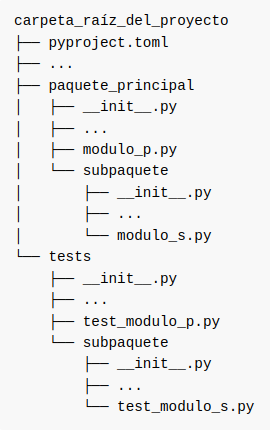
\includegraphics[width=0.5\linewidth]{logos/layout.png}
	\caption{Ejemplo de estructura plana.}
	\label{fig:layout1}
\end{figure}


Los paquetes implementados, sus módulos y la relación de uso entre ellos pueden observarse en el diagrama de la figura \ref{fig:modules1}.


\begin{figure}[h!]
	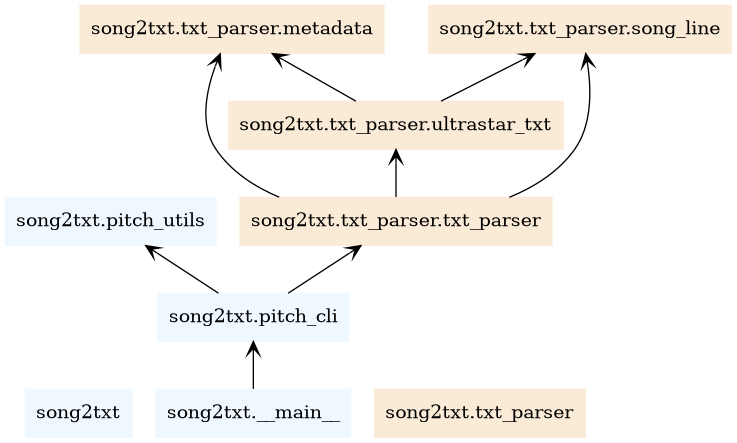
\includegraphics[width=\linewidth]{logos/packages.png}
	\caption{Diagrama de paquetes.}
	\label{fig:modules1}
\end{figure}


\subsection{Librería para trabajar con el formato UltraStar}
\label{sec:txtparser}

Para poder empezar a construir la aplicación es necesario poder trabajar con los archivos que definen las canciones de karaoke. Concretamente, con el formato de texto estándar UltraStar\footnote{\url{https://github.com/UltraStar-Deluxe/Play/wiki/UltraStar-txt-File-Format}},  compatible con la mayoría de videojuegos de karaoke como se puede observar en la sección \ref{sec:formatcomparison}.

Con esta intención, se ha construido una librería para leer este tipo de archivos transformando el texto a estructuras de datos apropiadas para trabajar con ellas y para escribir nuevos archivos generando el texto correspondiente a partir de las estructuras de datos.

\subsubsection{Lectura y decodificación}

En la definición del formato UltraStar no se establece la codificación de caracteres que deben usar los archivos, y como resultado, se comparten con distintas codificaciones. Tampoco es posible determinar la codificación a partir del archivo de forma sencilla, ya que son archivos de texto plano donde no se encuentra especificada.

Buscando la mayor compatibilidad se consideraron los siguientes acercamientos para decodificar los archivos:

\begin{itemize}
	\item{Probar a decodificar el texto por cada codificación posible hasta que todos los caracteres se descodifiquen sin ningún error.}
	\item{Estimar la codificación más probable para el contenido del archivo con una librería externa.}
	\begin{itemize}
		\item{Chardet}
		\item{cChardet}
		\item{Charset Normalizer}
	\end{itemize}
\end{itemize}

Inicialmente, se consideró la primera opción porque no añadía dependencias al proyecto. Sin embargo, era posible decodificar el texto sin errores, pero interpretando incorrectamente algunos caracteres (por ejemplo el carácter «ñ» podía ser interpretado incorrectamente como «ń»).

Por esta razón se decidió emplear el segundo enfoque con mayor fiabilidad. Teniendo en cuenta las pruebas de rendimiento disponibles en la \href{https://github.com/Ousret/charset_normalizer}{web} de Charset Normalizer y el tamaño de cada librería la opción más adecuada a las necesidades del proyecto es Charset Normalizer, ya que, presenta la mayor precisión y el menor tamaño de las opciones consideradas.

La implementación final estima el formato de codificación del archivo de texto entre varias opciones comunes (el formato estándar UTF-8 definido en la RFC 3629 \cite{rfc3629} y aquellos empleados por defecto en versiones antiguas del sistema operativo Windows). Si el texto sigue sin descodificarse correctamente, como último recurso, el usuario podría hacer uso de la utilidad de línea de comandos incluida en Charset Normalizer para transformar el archivo de texto a UTF-8 seleccionando manualmente la interpretación correcta.

\subsubsection{Diseño de las estructuras de datos}

Como plantillas para las estructuras de datos se han definido las clases representadas en la figura \ref{fig:class1}, intentando crear capas de abstracción adecuadas utilizando un modelado guiado por el dominio relativo al formato. Además, se han definido algunos comportamientos asociados:
\begin{itemize}
	\item{Comprobaciones de que los valores que se asignen son válidos (por ejemplo, la duración de una nota no puede ser negativa) tanto en creación como en modificación, en caso contrario, se indica el problema lanzando una excepción del tipo correspondiente con un mensaje que explica el error.}
	\item{Métodos para generar el texto que correspondería en un archivo UltraStar a partir de los datos almacenados en el objeto.}
	\item{Implementación del método \texttt{\_\_eq\_\_} para poder comparar objetos  y determinar si son iguales.}
\end{itemize}

\begin{figure}[H]
	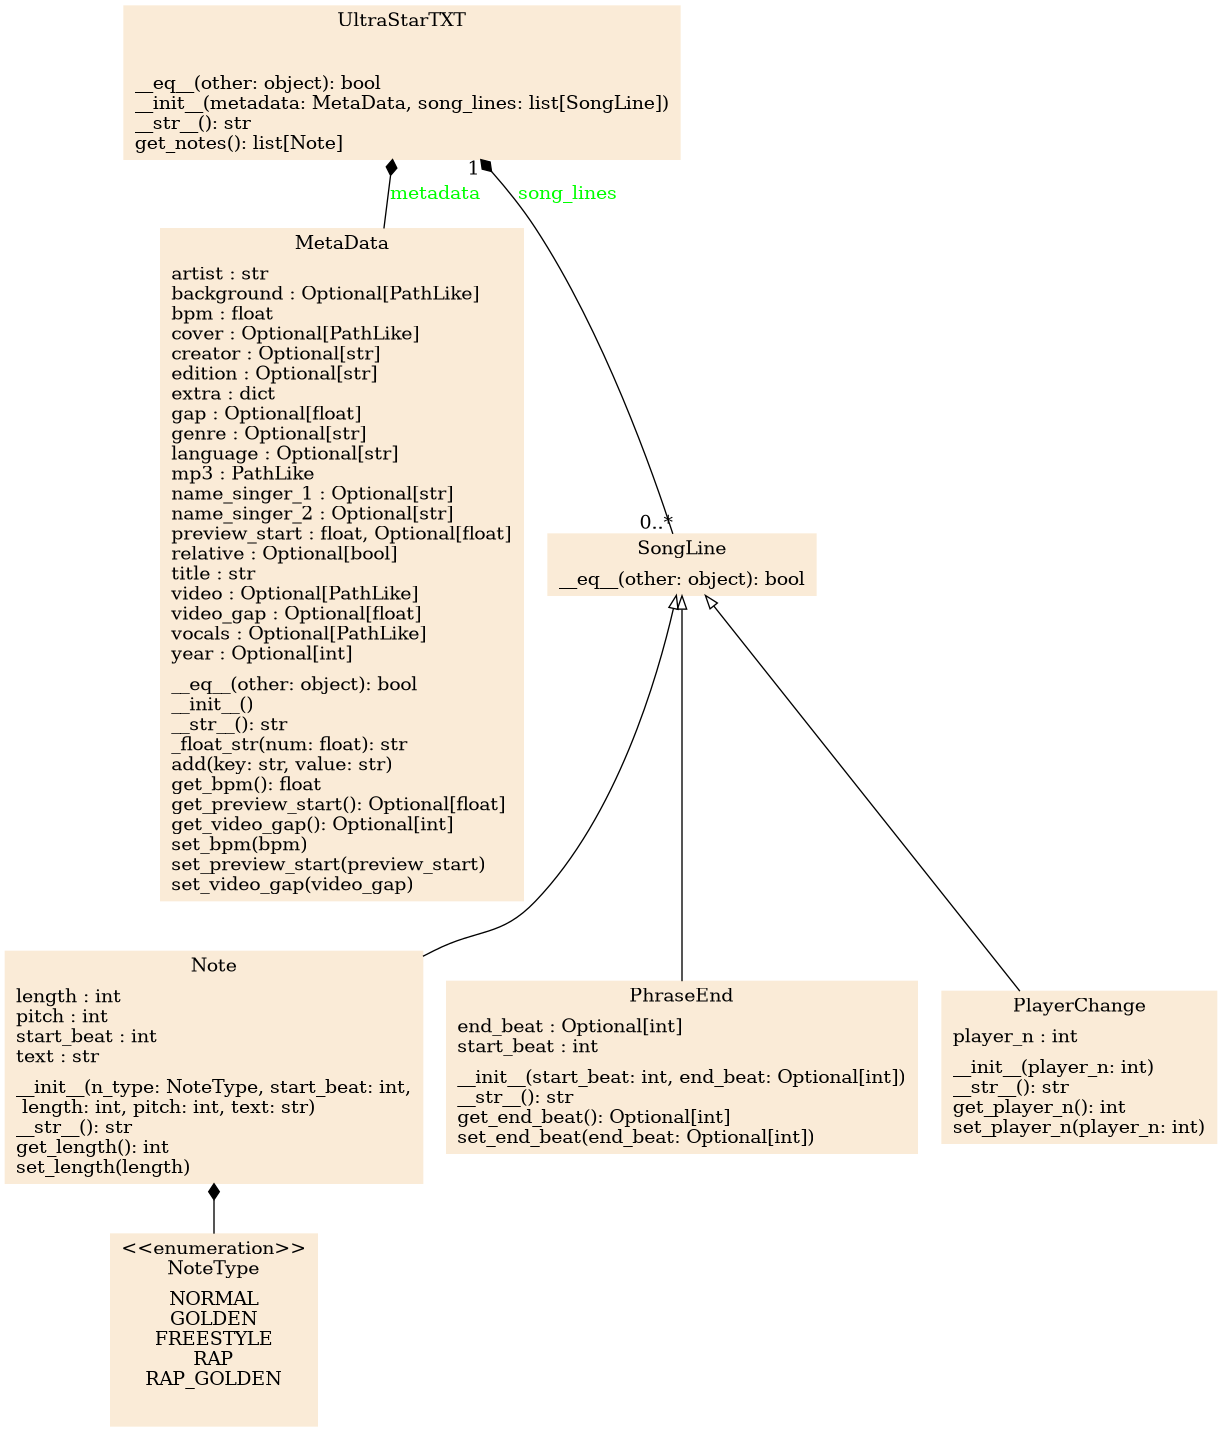
\includegraphics[width=\linewidth]{logos/classes.png}
	\caption{Diagrama de clases.}
	\label{fig:class1}
\end{figure}

\subsubsection{Transformación del texto a las estructuras de datos}

Se desea separar y extraer los fragmentos de texto que contienen la información relevante, para poder convertirlos a las estructuras de datos definidas. Buscando un método fácil de mantener y que permita garantizar que el texto de entrada presenta un formato correcto se han considerado las siguientes opciones:

\begin{itemize}
	\item{Operaciones básicas de transformación de texto, como separar por cada espacio, para quedarnos con una lista de los valores que necesitamos.}
	\item{Expresiones regulares para definir y detectar patrones.}
	\item{Módulos externos para generar un analizador del texto a partir de una definición de la gramática.}
\end{itemize}


Para escoger la opción más adecuada es importante tener en cuenta que el formato del texto presenta un lenguaje regular sencillo. Para este tipo de lenguaje las expresiones regulares son adecuadas permitiendo validar fácilmente que el texto presenta el formato correcto (a diferencia de las transformaciones básicas de texto) y siendo una solución corta, simple y precisa (a diferencia de los módulos de analizadores de propósito general, que son más adecuados para gramáticas complejas).

Por lo tanto, la implementación realizada procesa cada línea por orden utilizando expresiones regulares (ya que cada fragmento de información se encuentra separado en una línea distinta) y transforma la información extraída en objetos de las clases definidas anteriormente, componiendo finalmente un solo objeto que contiene toda la información del archivo de texto.  Si el formato del texto es incorrecto, ya sea por no respetar el orden (primero un bloque de metadatos, después descripción de la canción) o porque alguna línea no coincide con ninguna de las expresiones regulares, se lanza una excepción indicando el error y mostrando el número de línea que lo ha causado y su contenido.


\subsection{Lectura de archivos de audio}

Para poder estimar los tonos es necesario cargar el audio de la canción en una estructura de datos adecuada, específicamente un vector de muestras.

Idealmente, el programa debería soportar la mayor variedad de formatos posibles en múltiples plataformas. Concretamente, la compatibilidad con el formato MP3 es relevante debido a su omnipresencia. Sin embargo, como consecuencia de la existencia de patentes alrededor del formato que no expiraron hasta 2017\footnote{\url{https://www.tunequest.org/a-big-list-of-mp3-patents/20070226/}}, algunas librerías del sistema solo tienen soporte en las versiones más recientes (que una plataforma puede no haber recibido todavía).

Existen varias librerías de Python mantenidas activamente que permiten cargar audio en varios formatos (SoundFile, Pydub, audioread), sin embargo, todas dependen de librerías del sistema que el usuario puede no tener instaladas para decodificar formatos con compresión, como MP3. 

Otra opción, librosa, también depende de la existencia de una librería del sistema compatible para la lectura de audio, pero es capaz de trabajar con una amplia variedad, incluyendo todas las soportadas por el resto de opciones. Además, en sistemas operativos en los que no se encuentra ninguna de las librerías compatibles por defecto, se incluye una en la instalación.

Por lo tanto, como librosa satisface la compatibilidad con distintos formatos y plataformas sin necesidad de que el usuario instale software adicional manualmente, es la opción elegida para cargar el audio de la canción.

Adicionalmente, es una opción excelente para el proyecto, ya que, proporciona funciones relacionadas con el análisis musical, como estimación de las pulsaciones por minuto de la canción, transformación de hercios a tonos MIDI, normalización del audio y otras utilidades.

\subsection{Técnica para estimar frecuencias fundamentales}

La técnica usada para estimar la frecuencia fundamental de la voz debe tener la mayor precisión posible, teniendo en cuenta la rapidez con la que se completa la estimación como algo secundario. La precisión es la principal prioridad, ya que, es preferible que el creador de karaoke espere más tiempo a que tenga revisar manualmente las predicciones incorrectas.

Algoritmos clásicos como pYIN \cite{pYIN} son rápidos. Sin embargo, los enfoques utilizando redes neuronales, como CREPE \cite{CREPE} y SPICE \cite{SPICE}, han logrado mayor precisión como se puede observar en las figuras \ref{fig:crepecomparison} y \ref{fig:spicecomparison}.

\begin{figure}[h!]
	\centering
	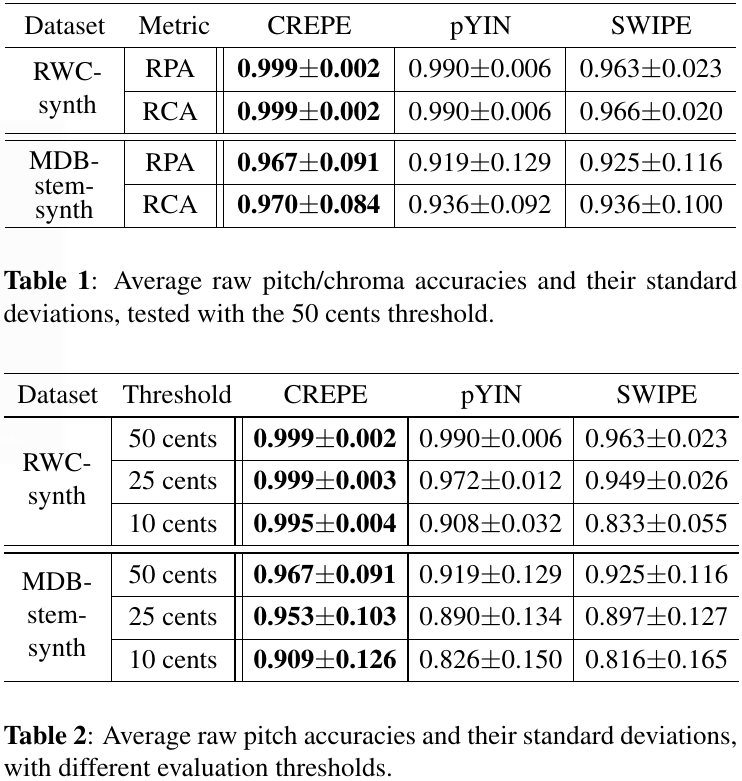
\includegraphics[width=0.7\linewidth]{logos/crepe_comparison}
	\caption{Comparación de CREPE con algoritmos clásicos\protect\footnotemark.}
	\label{fig:crepecomparison}
\end{figure}

\footnotetext{Imagen del repositorio de CREPE (\url{https://github.com/marl/crepe}) con licencia\texttt{ MIT}.}

En la figura \ref{fig:spicecomparison}, extraída del ensayo de SPICE, se puede observar como la precisión de CREPE y SPICE es muy similar, con una ligera ventaja de CREPE en el conjunto de datos de prueba que contiene más muestras con voz.

\begin{figure}[h!]
	\centering
	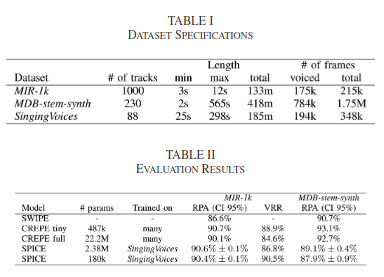
\includegraphics[width=0.7\linewidth]{logos/spice_comparison}
	\caption{Comparación de SPICE con CREPE\protect\footnotemark.}
	\label{fig:spicecomparison}
\end{figure}

\footnotetext{Imagen del ensayo de SPICE \cite{SPICE} con licencia \texttt{CC BY 4.0}.} 

Teniendo esto en cuenta, que CREPE ha recibido mejoras después de su publicación original\footnote{\url{https://pypi.org/project/crepe/}}, que provee modelos de distintos tamaños según la compensación de velocidad y exactitud deseada y que su integración en el proyecto es más sencilla, se considera CREPE el actual estado del arte y la opción elegida para estimar las frecuencias fundamentales.

\subsection{Cálculo de los tonos MIDI}

Para calcular los tonos es necesario conocer el intervalo de tiempo en el que se produce cada nota en la canción. Esto se puede obtener transformando la información extraída del archivo UltraStar, que nos proporciona la pulsación en la que empieza y cuantas pulsaciones dura cada nota, las pulsaciones por minuto \texttt{"bpm"} de la canción y el retraso de las notas respecto al inicio de la canción \texttt{"gap"} en milisegundos.

Teniendo en cuenta que las pulsaciones por minuto son multiplicadas por 4 para tener un posicionamiento de notas más preciso, la duración de una pulsación en milisegundos es:

\begin{displaymath}
	l = 60000 \frac{milisegundos}{minuto} \div (4bpm)\frac{pulsaciones}{minuto} = 15000 / bpm\frac{milisegundos}{pulsacion}
\end{displaymath}

Siendo 'x' el intervalo en pulsaciones e 'y' el intervalo en milisegundos:

\begin{displaymath}
	y_1 =  x_1 * l + gap
\end{displaymath}

\begin{displaymath}
	y_2 = x_2 * l + y_1
\end{displaymath}

Finalmente, para calcular los tonos de cada nota, se estiman las frecuencias en cada intervalo de tiempo utilizando CREPE, se hace la media descartando las predicciones que no superen la confianza mínima deseada, y se transforma las frecuencias obtenidas de hercios a MIDI utilizando librosa.


	% Conclusiones
	\chapter{Conclusiones y trabajos futuros}

\section{Conclusiones}

Con el trabajo realizado se ha conseguido avanzar en la creación automática de canciones para el formato UltraStar, cumpliendo el objetivo fijado para el proyecto.

Se ha contribuido al estado del arte, desarrollando la primera biblioteca pública en Python para trabajar con el formato UltraStar e implementando una aplicación para la asignación automática de tonos, que respecto a las existentes previamente: 

\begin{itemize}
	\item{Usa técnicas para la estimación de la frecuencia fundamental de mayor precisión, gracias a los avances recientes en redes neuronales.}
	\item{Provee una instalación más accesible con un empaquetado moderno, compatible con los principales sistemas operativos de escritorio y sin necesidad de instalar manualmente programas de terceros.}
	\item{Aporta documentación sobre los métodos empleados y las decisiones tomadas, tanto en esta memoria como en el propio repositorio donde se aloja la aplicación.}
\end{itemize}


Personalmente, la realización del trabajo ha servido no solo para demostrar habilidades adquiridas durante el grado, sino también como un vehículo para seguir aprendiendo sobre las apasionantes tareas propias de la creación de software eligiendo las soluciones más apropiadas.

Por último, me gustaría destacar la importancia del software libre, sin el cual este trabajo no habría sido posible, ya que ha sido crucial tanto en el aprendizaje como en el desarrollo, y, por tanto, la importancia de liberar el propio trabajo para facilitar futuras aportaciones.

\section{Trabajos futuros}

Alcanzar la automatización completa de las tareas descritas en la sección \ref{sec:problemdescription} está todavía muy lejos. Por ello, en contribuciones futuras se insta a seguir las siguientes líneas de trabajo:

\begin{itemize}
	\item{Desarrollar herramientas para obtener los metadatos de canciones a partir de servicios públicos en línea y guardarlos en el formato UltraStar (posiblemente haciendo uso de la librería implementada en este trabajo).}
	\item{Investigar e integrar soluciones para mejorar la precisión o la velocidad en la estimación de tonos, como:
	\begin{itemize}
		\item{Reducir la influencia de predicciones atípicas, ya sea haciendo la mediana de las predicciones en vez de la media u obviándolas si su desviación típica es demasiado alta.}
		\item{Utilizar técnicas del estado del arte para separar la voz del cantante del resto del audio previamente a la predicción, reduciendo así el ruido.}
		\item{Incrementar la precisión con nuevos modelos de redes neuronales o técnicas posteriores al desarrollo del proyecto, como\texttt{ HarmoF0}\cite{harmof0}.}
	\end{itemize}
	}
\end{itemize}


	
	\bibliography{bibliografia}
	\bibliographystyle{plain}
	
\end{document}

